\section{Processing an image by 2D Maximum Likelihood}

Maximum likelihood (ML) processing is available in {\twodx}\texttt{\_image} for two-dimensional alignment. This is a refinement process which should be performed after the unbending process. The corresponding script is called \textit{ML-2D (for advanced users)} and can be found in the Standard Script panel. The density map shown in \autoref{fig:2dml_start} shows the result obtained without maximum likelihood refinement.

For detailed information we refer to \cite{ml1}. Note that using this module is not trivial. Here we are just focusing on the GlpF test data set. In order to conduct the ML processing, you first need to set up related parameters. You can right click on a parameter to view the description. Some tips are provided to help you decide the parameter values. 

\begin{figure}[H]
	\centering
	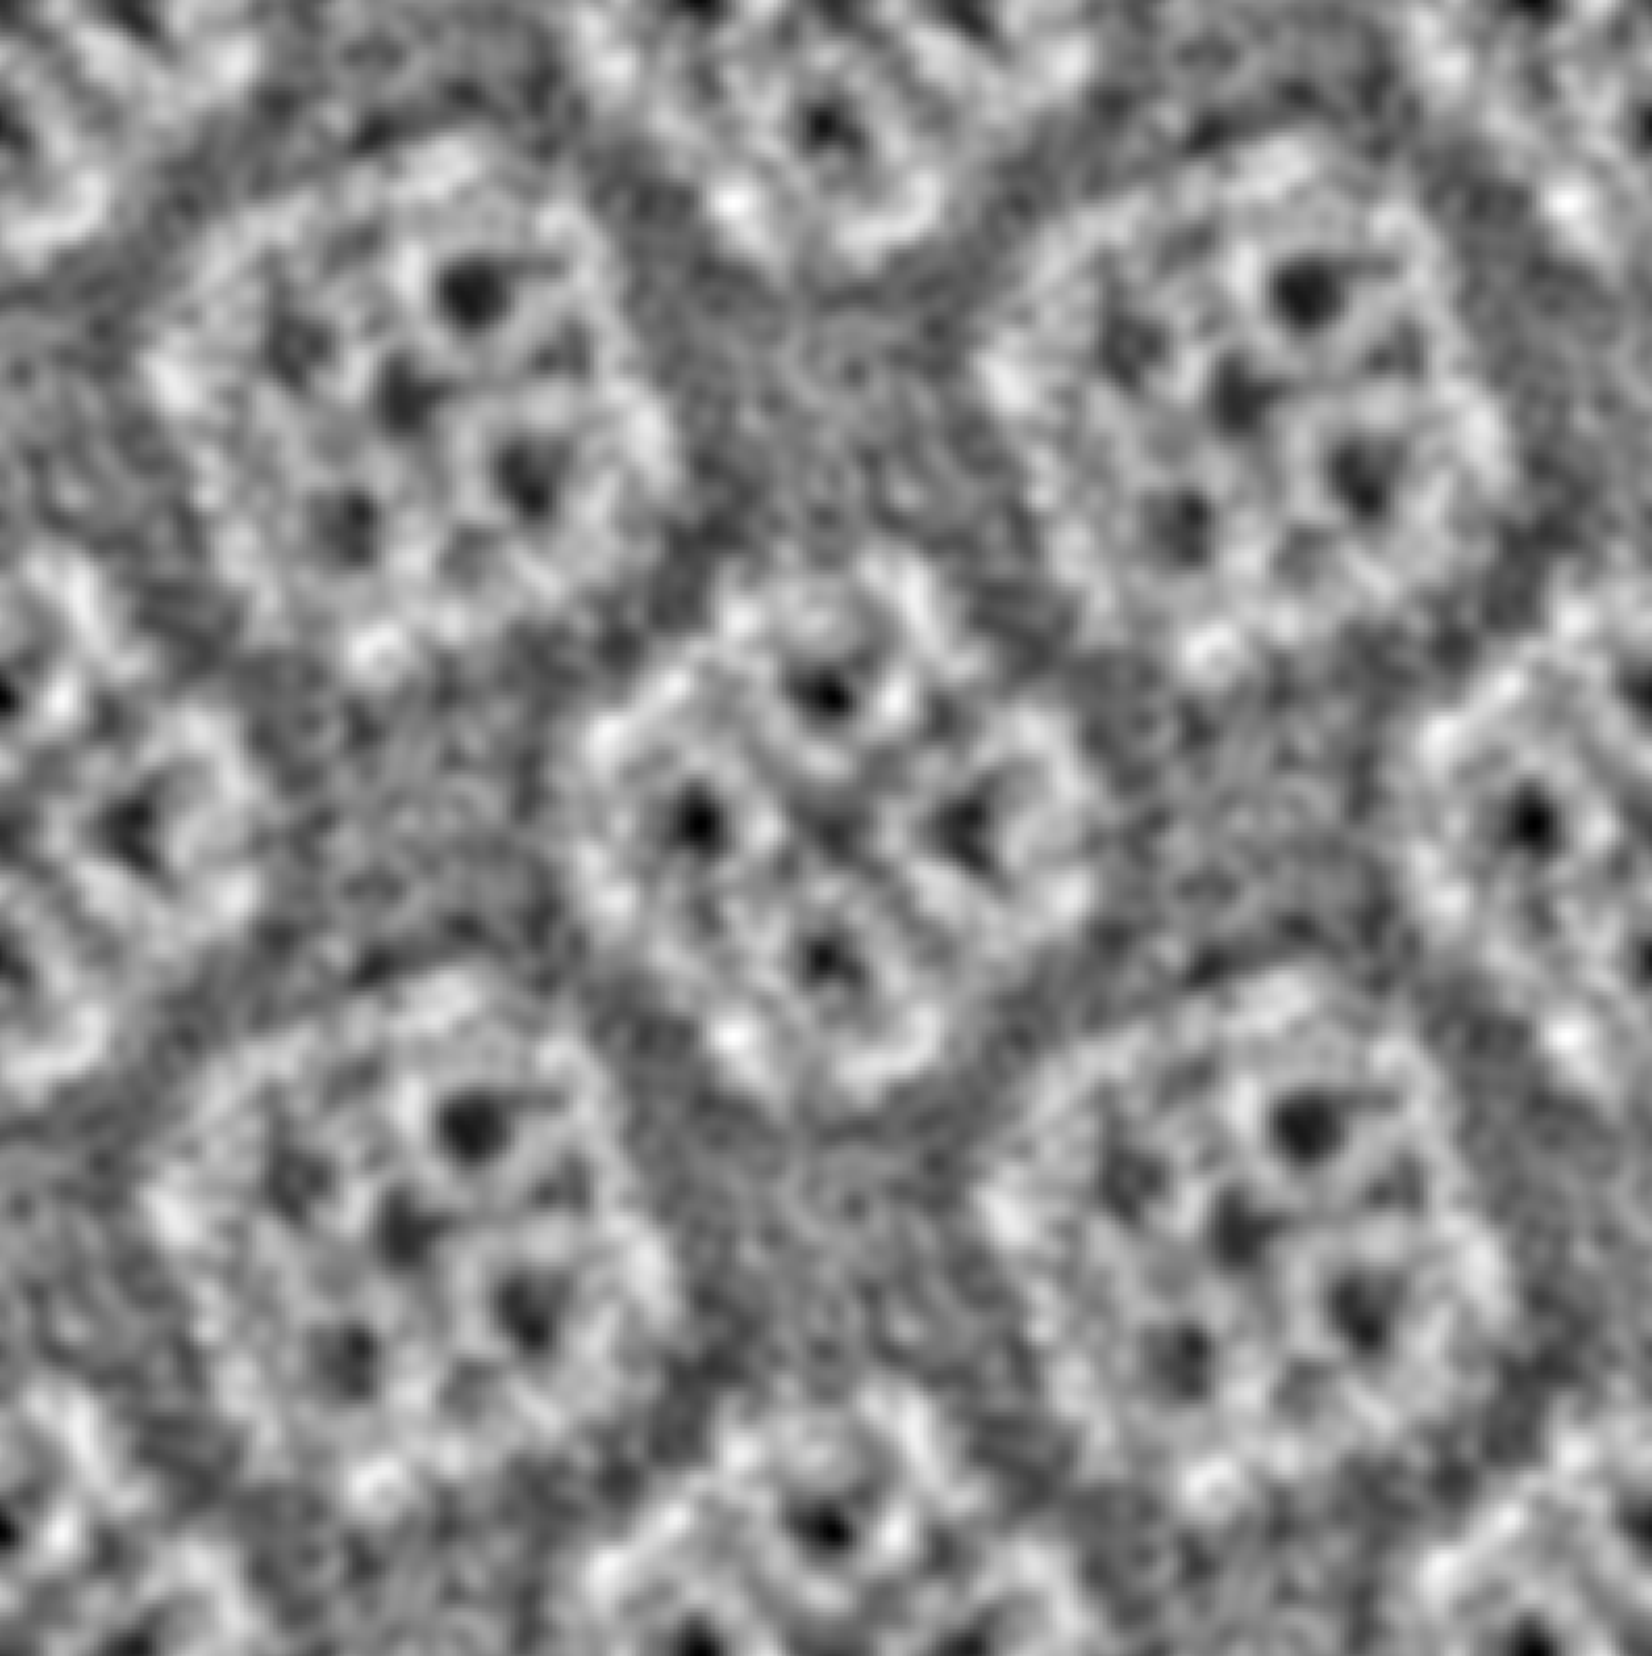
\includegraphics[width=0.45\textwidth]{2dml_start.pdf}
	\caption{Map before ML}
	\label{fig:2dml_start}
\end{figure}

\begin{enumerate}
	\item Set \textit{Process Single Particle Reconstruction} to \textit{Yes} in the \textit{Maximum Likelihood Algorithm} section in the Parameter panel in order to activate the maximum likelihood refinement in {\twodx}. If you run the script without this option nothing will happen.
	
	\item Select \textit{Maximum Likelihood Calculation} for the \textit{Weighting profile from} in the same section of the Parameter panel.
	
	\item Set the \textit{Total Diameter of the windows} to a size that is larger than the unit cell. You find this option in the \textit{Maximum Likelihood Parameters} section of the Parameter panel. For the test dataset we recommend around $1.2$ times of the unit cell size, i.e. $120, 120$.
	
	\item Set the \textit{Diameter of the circular mask} to a size that is slightly larger than the unit cell. In our case we used $110$.
	
	\item In most cases, select \textit{relative percentage given} for \textit{Threshold determination method for particle selection}, and set the relative percentage to your needs.  A value of $50$ means the top $50$\% particles will be used in the ML processing. The particles are extracted from the cross-correlation profile generated during the \textit{Unbend I} script.
	
	\item Select \textit{Gaussian} as \textit{Type of low-pass filter}.
	
	\item Set \textit{Low-pass filter radius} to a value between $0.25$ and $0.5$. In our test case we use $0.25$.
	
	\item Set \textit{Apply noise whitening} to \textit{Yes} in order to enable noise whitening which improves the convergence of the maximum likelihood method.
	
	\item Set \textit{Apply CTF correction} to \textit{Yes} to correct for the contrast transfer function for each particle.
	
	\item Set up \textit{Angular range} and step for angle search. For well ordered crystals, you can use a smaller range.  If you don't want to do angle search, use 0 for range. The step size must always be positive (nonzero). For the test dataset we used $-10$ to $10$ degrees with a step size of $1.0$.
	
	\item Set \textit{Terminate after maximum number of iterations} to a value usually between $20$ and $40$.
	
	\item Set \textit{Termination if change in dev\_sigma or dev\_sigma\_theta below} to a small positive number less than $0.1$.
	
	\item \textbf{Before running the script click on save in the header panel, otherwise your parameter will not be applied}. After setting up and saving the ML related parameters, you click on \textit{ML-2D} in the Standard Scripts panel to launch the process. You can view the results by clicking on reference maps listed in the Images panel. \autoref{fig:2dml_result} shows our 2D maximum likelihood results.
	
	\begin{figure}[H]
		\centering
		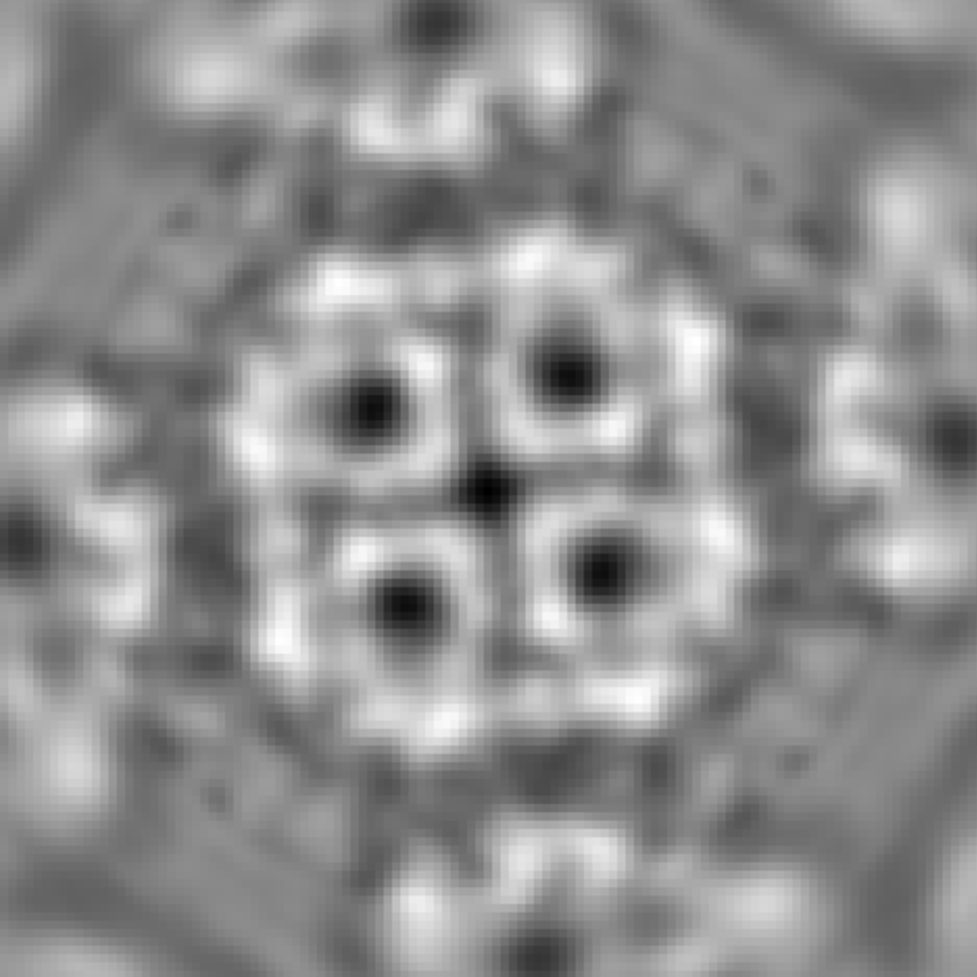
\includegraphics[width=0.45\textwidth]{2dml_result.pdf}
		\caption{Map after ML}
		\label{fig:2dml_result}
	\end{figure}

\end{enumerate}